\documentclass[10pt]{article}
\usepackage{amsmath}
\usepackage[dvipsnames]{xcolor}
\usepackage{subcaption}
\usepackage{graphicx}
\usepackage{algorithm}
\usepackage[noend]{algpseudocode}
\floatname{algorithm}{Algorithm}
\usepackage{hyperref}
\usepackage[capitalise, noabbrev]{cleveref}
\newcommand{\todo}[1]{{\color{red}#1}}

\algblock[TryCatch]{try}{endtry}
\algcblockdefx[TryCatch]{TryCatch}{catch}{endtry}
	[1]{\textbf{catch} #1}


%% ----------------------------------------------------------------

\title{
    Othello \\
    \vspace{3em}
    {\large Umeå University \\
    Artificial Intelligence - Methods and Applications (5DV181)}
    \vspace{3em}
    
}
\author{Salome Müller, mcs21smr}
\date{\today}

\begin{document}

%% Make the title
\maketitle

\vspace{1em}

%% Write the abstract
\begin{figure}[h]
    \centering
    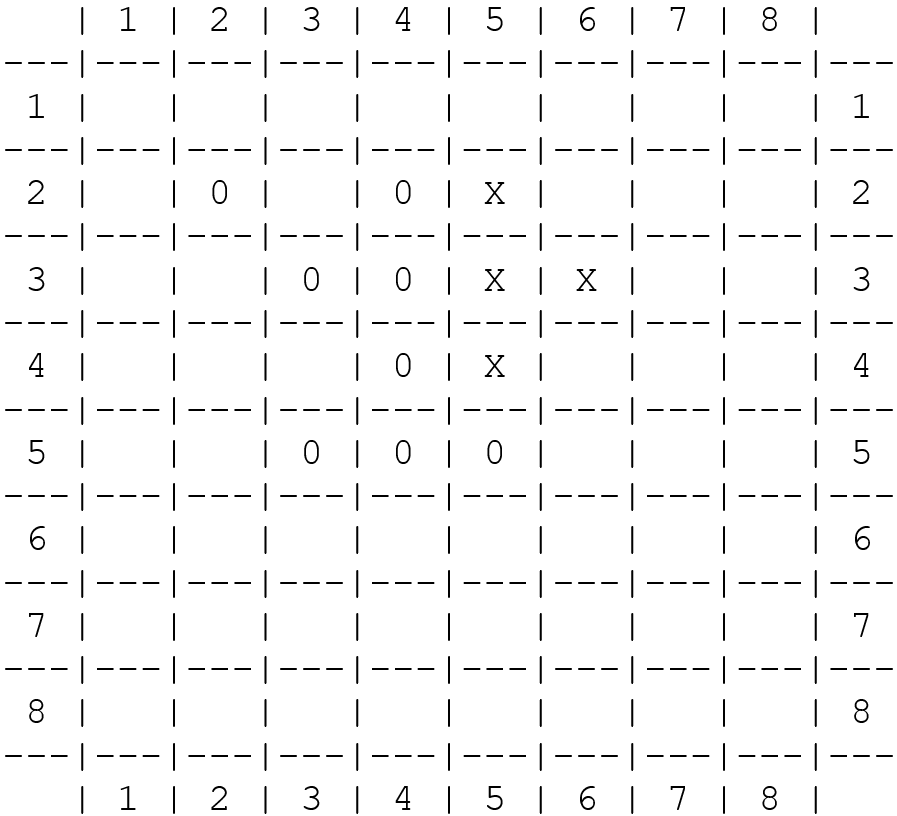
\includegraphics[width=0.7\textwidth]{position1.png}
\end{figure}

\pagebreak

%% Include all chapters
\section{Introduction}

Othello is a board game for two players, \textit{white} and \textit{black}.
In turns they can place pieces of their color on the board, an change the color of some of the pieces already there.
In the end, the player with more pieces wins.

Using Java we implement an engine that suggests a move, given the configuration of the board and the player, within a given time limit.
The engine uses an alpha-beta search algorithm and a compound heuristic, combining a score and a mobility heuristic.
With this heuristic and a time limit of two seconds per move, a naive opponent using the score heuristic and search depth seven can be defeated.

This report is structured into two sections.
In \cref{sec:implementation} the implemented methods and algorithms are explained, as well as the heuristic.
Further, we explain how to install and run the program.
\cref{sec:evaluation} evaluates the different heuristics for both players and different time limits.

\section{Implementation}
\label{sec:implementation}
In this section we go into detail about the implementation, before we explain how the program can be installed and used.
We describe the game, the used search algorithm, alpha-beta, the different heuristics and the main functionality.

\subsection{Othello Board}
Othello is a board game, where two players, \textit{black} and \textit{white}, in turn place stones of their respective color on a $8\times 8$ board.
The stones are black on one site and white on the other, so that they can be flipped to show the other color.
Each move consists of placing a stone on the board and then adapting the pieces on the board according to that stone.
All the opponent's stones may be turned, that lie on a straight line between the placed stone and another stone of the players color.
One example for this can be seen in~\cref{fig:boards}, where one player places a stone in field (4, 3), which allows them to flip the blue colored stones.
If no stone can be placed such that stones can be turned, the player must pass this move.
The game is over, as soon as no player can make another move, and the player with more stones on the board wins.
The board is then in a terminal position.

\begin{figure}[!ht]
    \centering
    \begin{subfigure}[b]{0.48\textwidth}
        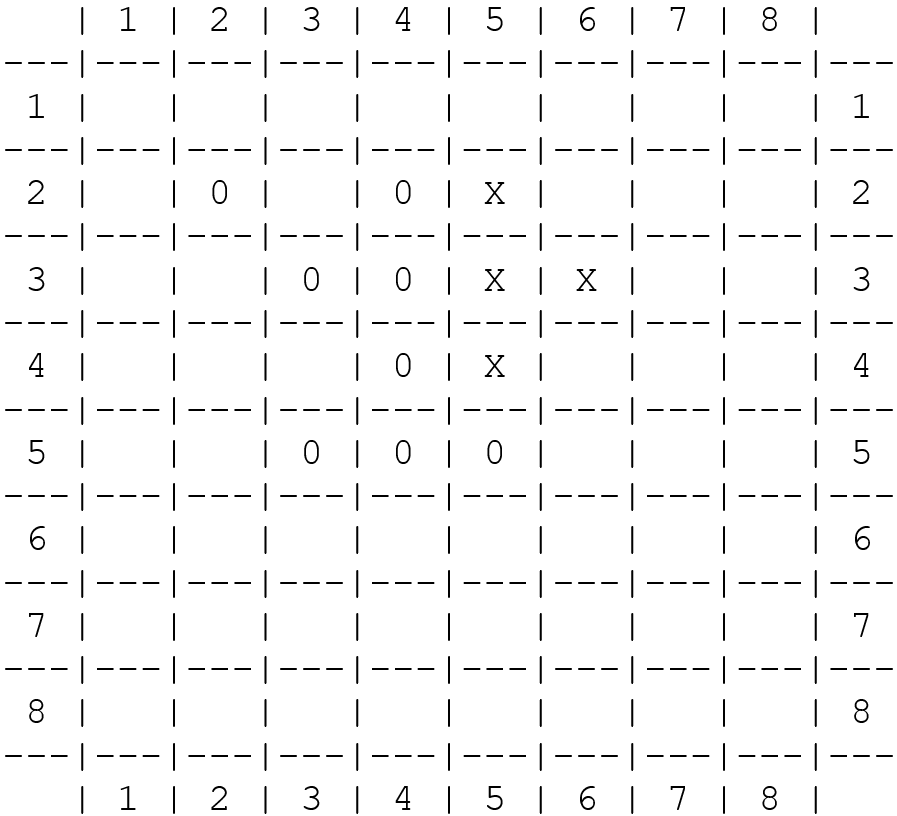
\includegraphics[width=1\textwidth]{position1.png}
    \end{subfigure}
    \hfill
    \begin{subfigure}[b]{0.48\textwidth}
        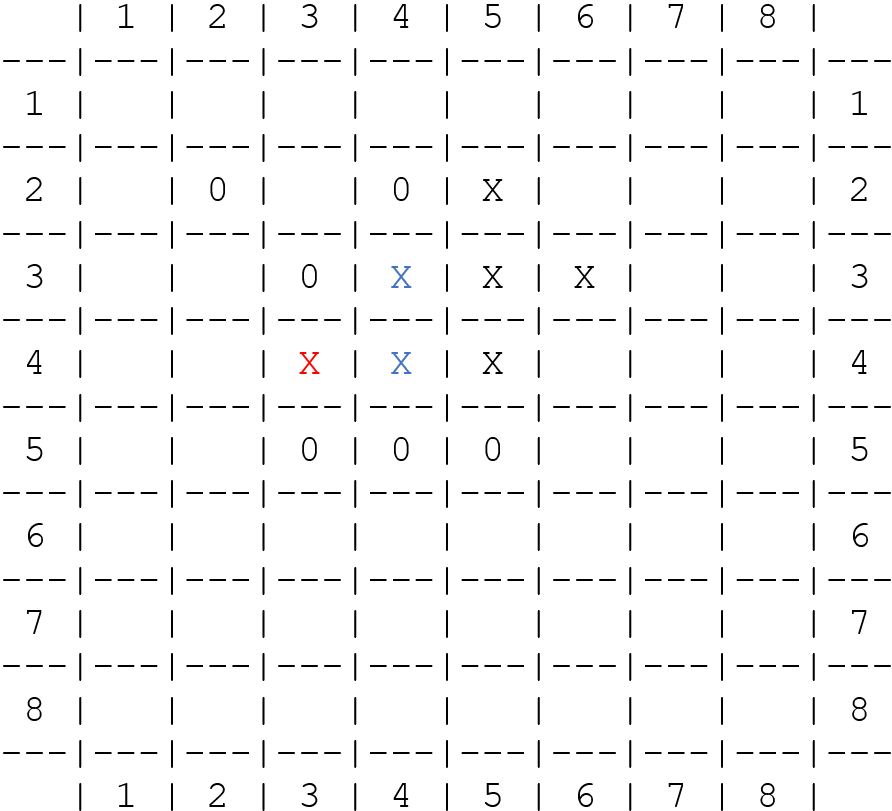
\includegraphics[width=1\textwidth]{position2.png}
    \end{subfigure}
    \caption{Two Othello positions. The right board is the result of placing a stone in column 3, row 4 (red) and flipping the respective stones (blue).}
    \label{fig:boards}
\end{figure}

We implemented the game in two parts: one representing the board, the other an action a player could perform, \texttt{OthelloPosition} and \texttt{OthelloAction} respectively.
\texttt{OthelloPosition} holds the board represented as a a $10\times 10$ matrix of characters, where the actual board is in the center of the array.
The two additional rows and columns are used to prevent \texttt{array-out-of-bound}-exceptions and thus make some computations easier.
Using this array, the class can generate a list of all possible moves for the current player and apply one of those moves.
The latter of those methods is called \texttt{makeMove} and takes an \texttt{OthelloAction} as input.
It does not change the position, but creates an exact copy of it.
On this copy, the action is applied and the resulting configuration of the board is returned, i.e., all required stones are turned and the player is set to the next player.

To find the best move in the list of possible moves, we evaluate them with an alpha-beta search.

\subsection{Alpha-Beta Search}
Alpha-beta search is a type of adversarial search.
These search algorithms try to find the best of multiple options, in our case moves, assuming that the adversary always chooses their best option.
For this, we generate an (implicit) game tree.
Each node represents one configuration of the board together with the information whose turn it is.
The children of one node are exactly the configurations that can be reached with one move of the current player.
The right board in~\cref{fig:boards} is one of many children of the left board.
If a leaf is reached, i.e., a terminal position, the score is calculated.
It is calculated in a way that it is positive if \textit{white} wins and negative if \textit{black} wins, i.e., $score = |\text{white pieces}| - |\text{black pieces}|$.
\textit{White} will always choose the move leading to its child with the highest value among all its children, while \textit{black} does the opposite.
The according algorithm is called minimax-algorithm.

If time and space were not limited, we could search the whole tree and would find the best  move.
However, this is not the case, and since branching factors and the search depth are high, it is not feasible to search the whole tree.
In fact, the branching factor is ten in average and the depth is up to sixty, as sixty pieces can be placed on the board.
The number of nodes thus lies in $O(10^{60})$.
Therefore, we use an algorithm that prunes the search tree.

The algorithm for alpha-beta search uses two additional values, $\alpha$ and $\beta$.
They are used to identify branches of the search tree which result in values, that will never be used.
These branches are then pruned.
In the best case, this reduces the number of nodes that need to be considered to $O(\sqrt{10^{60}})$, which is still too big to search the tree within the given time limit.
Therefore, we additionally use a fixed search depth.
When a node of this depth is reached in the search tree, the node's value is evaluated with a heuristic.
Since we do not know how deep we can get within the time limit, we start with depth one and increase the depth iterative.
When the time is up, we use the action that was found within the last completed search.

Alpha-beta search is traditionally implemented with two different functions, \texttt{maxValue} and \texttt{minValue}, that call each other alternately.
\cref{alg:max} shows \texttt{maxValue}, \texttt{minValue} is symmetric to it.

\begin{algorithm}[H]
    \caption{Alpha-Beta Search}
    \label{alg:max}
    \begin{algorithmic}[1]
        \Function{maxValue}{OthelloPosition position, int $\alpha$, int $\beta$, int depth}
            \If{time\_is\_up}
                \State stop\_execution;
            \EndIf
            \If{depth = 0}
                \State \textbf{return} $h(\text{position})$;
            \EndIf
            \If{position.is\_final\_position()}
                \State position.change\_player();
                \State \textbf{return} position.score();
            \EndIf
            \State
            
            \State moves $\leftarrow$ position.get\_moves();
            \If{$|$moves$|$ = 0}
                \State \textbf{return} min\_value(position, $\alpha$, $\beta$, depth - 1); /*\emph{pass move}*/
            \EndIf

            \State value $\leftarrow -\infty$;
            
            \For{move $\in$ moves}
                \State new\_position $\leftarrow$ position.make\_move(move);
                \State new\_value $\leftarrow$ min\_value(new\_position, $\alpha$, $\beta$, depth - 1);
                \State value $\leftarrow$ max(new\_value, value);
                \State $\alpha$ $\leftarrow$ max(new\_value, $\alpha$);
                \If{$\alpha$ $\geq$ $\beta$}
                    \State break; /*\emph{$\beta$-cutoff}*/
                \EndIf

            \EndFor 
            
            \State \textbf{return} value;
        \EndFunction
    \end{algorithmic}
\end{algorithm}

This function returns the value of the best action, but not the action itself, as it is more efficient to return integer values instead of \texttt{OthelloAction} objects.
Since we need the action, we add two more methods, \texttt{initialMinValue} and \texttt{initialMaxValue}.
When the search is started, depending on whose turn it is, either \texttt{initialMaxValue} (\textit{white}) or \texttt{initialMinValue} (\textit{black}) is called.
These two methods return the action with the highest or lowest value respectively.
\texttt{initialMaxValue} can be seen in \cref{alg:initMax}, \texttt{initialMinValue} is, again, symmetric to it.

\begin{algorithm}[H]
    \caption{Alpha-Beta Search Initialisation}
    \label{alg:initMax}
    \begin{algorithmic}[1]
        \Function{initalMaxValue}{OthelloPosition position, int depth}
            \State moves $\leftarrow$ position.get\_moves();
            \If{$|$moves$|$ = 0}
                \State \textbf{return} new OthelloAction(\lq pass\rq);
            \EndIf

            \State value $\leftarrow -\infty$;

            \For{move $\in$ moves}
                \State new\_position $\leftarrow$ position.make\_move(move);
                \State new\_value $\leftarrow$ min\_value(new\_position, $\alpha$, $\beta$, depth - 1);
                \If{new\_value $>$ value}
                    \State best\_move $\leftarrow$ move;
                    \State value $\leftarrow$ new\_value;
                    \State $\alpha$ $\leftarrow$ max(new\_value, $\alpha$);
                \EndIf
            \EndFor 
            
            \State \textbf{return} best\_move;
        \EndFunction
    \end{algorithmic}
\end{algorithm}

The heuristic to be used is assigned to the algorithm before starting the search.
We next introduce the heuristics we use in the evaluation.

\subsection{Heuristics}
We used two different heuristics, as well as the combination of those two heuristics.
The first heuristic is a naive approach counting the stones on the board while the second one returns a value for the mobility.

\paragraph{Naive Heuristic}
The naive heuristic of a position is equal to the score which would be achieved, if the position was a terminal position.
\[h_{n}(p) = |\text{white pieces}| - |\text{black pieces}|\]

\paragraph{Mobility Heuristic}
The mobility heuristic is a normalized value for the mobility of the two players.
It is calculated using the number of moves a player could perform on the position.
\[h_{m}(p) = 64 * \frac{|\text{white moves}| - |\text{black moves}|}{|\text{white moves}| + |\text{black moves}|} \]

If the sum of both moves is zero, i.e., no player can make a move, we return the score of the board instead.
We normalize the heuristic value to the range [-64, 64], in order to align it to the end scores

\paragraph{Compound Heuristic}
We compound the two former heuristics to one heuristic by taking the weighted sum of both.
The weight assigned to each heuristic depends on how far into the game the evaluated position is, which we estimate from the number of empty fields.
\begin{align*}
    w &= \frac{|\text{empty fields}|}{64} \\
    h_{c}(p) &= w * h_{m}(p) + (1 - w) * h_{n}(p)
\end{align*}


\subsection{Time Limit}
The time available for the search is limited by a given number of seconds.
At the beginning of the program, we calculate the timestamp of when the program must terminate.
The iterative deepening of the algorithmic search is performed in a conditional while loop, as can be seen in~\cref{alg:time} on Line 6.

\begin{algorithm}[H]
    \caption{Iterative Deepening}
    \label{alg:time}
    \begin{algorithmic}[1]
        \Function{Othello}{OthelloPosition position, int timeLimit}
            \State endTime $\leftarrow$ currentTime + timelimit;
            \State algorithm $\leftarrow$ new OthelloAlgorithm();
            \State action $\leftarrow$ null;
            \State executorService $\leftarrow$ new SingleThreadExecutor(); \label{lst:service}
            
            \While{currentTime $<$ endTime} \label{lst:while}
                \State algorithm.increaseSearchDepth();
                \State future $\leftarrow$ executorService.start(algorithm.search()); \label{lst:future}
                \try
                    \State action $\leftarrow$ future.get(endTime - currentTime);
                \catch{TimeoutException}
                    \State algorithm.interrupt(); \label{lst:interrupt}
                \endtry
            \EndWhile 
            
            \State \textbf{return} action;
        \EndFunction
    \end{algorithmic}
\end{algorithm}

At each iteration the search depth is increased, and the search is started in a separate thread.
For this, the Java \texttt{ExecutorService} class is used (Line 5).
This service allows to start a callable function concurrently in another thread (Line 8).
By using Java's \texttt{Future} class, the function's result can be retrieved as soon as the task is done (Line 8).
If the time limit is reached before the task is done, an exception is thrown.
In that case, we safely stop the thread by interrupting the search algorithm (Line 12).
Otherwise, the search could be terminated correctly, and the retrieved move is assigned to \texttt{action}.

The class \texttt{OthelloAlgorithm} holds a Boolean \texttt{interrupted}, which is \textit{false}.
\texttt{algorithm.interrupt()} (Line 12) sets \texttt{interrupted} to \textit{true}.
When \texttt{minValue} and \texttt{maxValue} are called, they first check whether \texttt{interrupted} is \textit{true}.
If it is, an \texttt{InterruptedException} is thrown, which forces this thread to terminate with an error.
This behaviour is unconventional, but since we do not care about any value from this search, this does not matter.
We use the last found action, which is not affected in any way by the interrupted search, and require the search thread to stop immediately.

\subsection{Installation and Usage}
The program's source code can be downloaded from \href{https://github.com/muesal/othello}{GitHub}.
After the download the code can be compiled with \texttt{javac Othello.java} and executed with \texttt{java Othello <board> <time>}.
\texttt{board} should be a string of length 65, the first character being either \lq\textit{W}\rq~or \lq\textit{B}\rq~indicating whose turn it is, followed by the configuration of the board.
The board has 64 fields, each can be either empty (\lq\textit{E}\rq) or contain a white (\lq\textit{O}\rq) or black (\lq\textit{X}\rq) stone.
\texttt{time} is the time limit in seconds.
The program will run for no longer than the given amount of seconds.

The repository further contains a bash script, \texttt{othello.sh}, which takes the same input arguments and a flag for whether or not the code should be compiled first.
This script can be used to simulate a whole game, e.g., by using \texttt{test\_code/othellostart} with two scripts like \texttt{othello.sh} and a time limit.

\section{Evaluation}
\label{sec:evaluation}

We test our implementation by playing against an agent who uses the naive heuristic and a search depth of seven.
We evaluate all three heuristics with time limits 2, 4, 6, 8 and 10 seconds.
The given time limit is strictly adhered to, the average time per move over a game is about 0.2 seconds lower than the limit (e.g., 5.8 s for a limit of 6 s).

\subsection{Naive Heuristic}

As can be seen in~\cref{tab:naive}, the naive heuristic is sufficient to win against the other agent, even though they use the same heuristic.
This is mainly due to the fact that we use iterative deepening and thus reach higher search depths.
Our implementation can reach depths ten (2 s) or eleven (10 s).

\begin{table}[!ht]
\centering
\begin{tabular}{ |c||c|c|c||c|c|c| } 
 \hline
 Time & Player & Won & Score & Player & Won & Score \\ \hline \hline
  2 & White & Yes & 16 & Black & Yes & -16 \\ 
  4 & White & Yes & 36 & Black & Yes & -35 \\  
  6 & White & Yes & 36 & Black & Yes & -48 \\  
  8 & White & Yes & 38 & Black & Yes & -56 \\   
 10 & White & Yes & 64 & Black & Yes & -56 \\ 
 \hline
\end{tabular}
\caption{\label{tab:naive} End scores for different time limits when playing as \textit{white} or \textit{black} using the naive heuristic.}
\end{table}

This heuristic is good when a high search depth can be reached.
In this case, the heuristic is evaluated on positions which are terminal positions or close to one.
However, if the search can not go deep and is evaluated on earlier positions of the board, the heuristic value is not reliable, since the board changes a lot in the course of the game.
If a player has a lot of stones in the beginning this does not necessarily mean that they will have a lot of stones in the end.


\subsection{Mobility Heuristic}
\cref{tab:mobil} shows the results when using the mobility heuristic.
This heuristic is more computationally complex than the naive heuristic, therefore only depths eight and nine could be reached.
This heuristic is a lot better for \textit{black} than for \textit{white}, which shows that this heuristic is not reliable on its own.

\begin{table}[!ht]
\centering
\begin{tabular}{ |c||c|c|c||c|c|c| }
 \hline
 Limit & Player & Won & Score & Player & Won & Score \\ \hline \hline
  2 & White & Yes &  30 & Black & No  & 2 \\ 
  4 & White & No  & -41 & Black & Yes & -12 \\  
  6 & White & No  & -12 & Black & Yes & -50 \\  
  8 & White & No  & -14 & Black & Yes & -50 \\   
 10 & White & No  & -13 & Black & Yes & -50 \\ 
 \hline
\end{tabular}
\caption{\label{tab:mobil} End scores for different time limits when playing as \textit{white} or \textit{black} using the mobility heuristic.}
\end{table}

Opposed to the naive heuristic, the mobility heuristic is assumed to be better for earlier positions.
In the beginning, it may be better to try and restrict the opponents possibilities.
However, the quality of the moves is of more importance than their quantity which is why this heuristic does not yield good results.


\subsection{Compound Heuristic}
The best results were achieved with the compound heuristic, even though only depths eight end nine could be reached.
As can be seen in~\cref{tab:comp}, when playing as \textit{white} we win with more than sixty points for every time limit and with more than forty points when playing as \textit{black}.
Despite the fact that the mobility heuristic on its own is not satisfactory, it improves the naive heuristic when they are used together, as the reached scores are better.

\begin{table}[!ht]
\centering
\begin{tabular}{ |c||c|c|c||c|c|c| } 
 \hline
 Limit & Player & Won & Score & Player & Won & Score \\ \hline \hline
  2 & White & Yes & 62 & Black & Yes & -42 \\ 
  4 & White & Yes & 64 & Black & Yes & -45 \\  
  6 & White & Yes & 62 & Black & Yes & -46 \\  
  8 & White & Yes & 62 & Black & Yes & -62 \\   
 10 & White & Yes & 64 & Black & Yes & -61 \\ 
 \hline
\end{tabular}
\caption{\label{tab:comp} End scores for different time limits when playing as \textit{white} or \textit{black} using the compound heuristic.}
\end{table}

An agent using this heuristic uses the best of $h_{n}$ and $h_{m}$.
In the beginning, when the board is almost empty, the agent tries to restrict the other player's possibilities.
With time, while the board is being filled, the agent shifts it's focus to yielding a high score.
Hence, the mobility becomes negligible, while the importance of the amount of stones on the board increases.

\section{Conclusion}

Implementing a search algorithm for Othello, we looked at three different heuristics.
Two can beat an agent using the naive heuristic, namely the naive heuristic itself and a compound heuristic using the naive and the mobility heuristic.
The mobility heuristic on its own is not considered suitable as heuristic, as it does not yield good results.

Our implementation of alpha-beta search runs on an implicit search tree, i.e., the nodes are not stored but computed from their parent, and forgotten after evaluating them.
If a further speed up were necessary to win, the tree could be built explicitly and stored between the iterations.
This way, the moves would only have to be computed and applied once per position.
Further, at iteration $k$, we could order the children of a node according to their value at iteration $k-1$ and then evaluate them in this order.
This way, better moves would be more likely to be evaluated first, and more parts of the tree could be pruned.

However, winning within the time limit was not a problem, as this was easily done with the naive heuristic.
Initially, after printing the chosen action the program continued the last search until it was finished, leading it to exceed the time limit.
Java does not feature a way to kill a thread, so no Java built-ins could be used to solve this problem.
This could eventually be resolved by throwing an \texttt{InterruptedException} in the search thread, which kills the thread immediately.


\end{document}